\section{Tilstandsmaskin}
\thispagestyle{fancy}

Etter at IEC blokkene var ferdige var det naturlege neste steget å begynne på tilstandsmaskina som skulle styre sjølve SBR-prosessen
og styringa av anlegget. Vi hadde allereie danna oss eit bilete, men kunne no byrja og bruke kunnskapen frå verkemåten til anlegget
til å grovt fylle inn dei hendelsane og aksjonane som foregikk mellom tilstandsbytter. 
Tilstandsmaskina er bygd opp av dei fem reaktortilstandane som førekomer i eit SBR-anlegg.

Dette er ein enkel modell av korleis tilstandsmaskina er programmert men gir eit godt innblikk i systemet.

\begin{figure}[htbp]
    \centering
    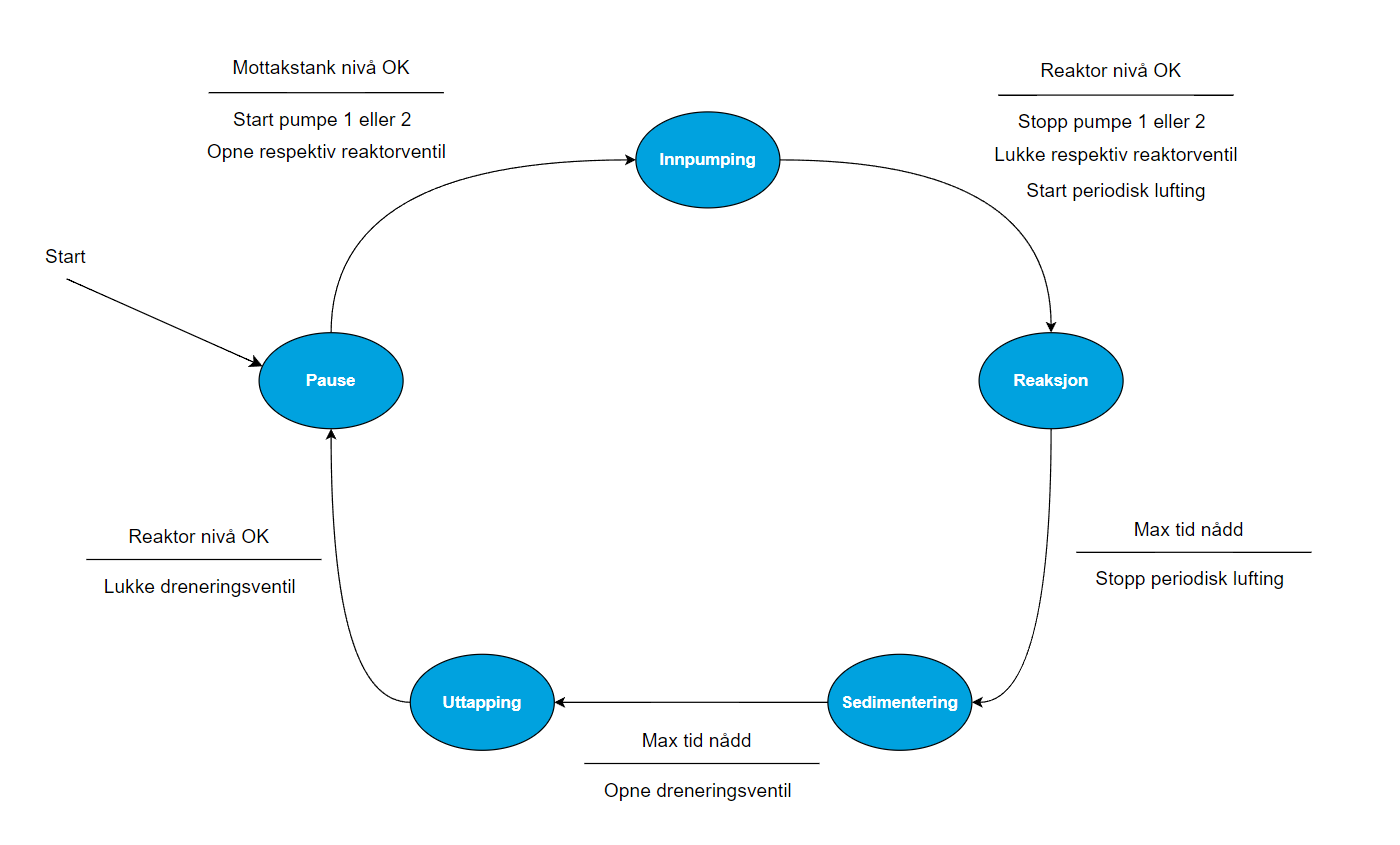
\includegraphics[width=1\textwidth]{Figurar/Simpel tilstandsmaskin.png}
    \caption{Simpel model av tilstandsmaskin}\label{fig:reaktorsoner}
\end{figure}

Utifrå det vi allereie hadde lært om anlegget visste vi kva inngangssignalar og logikk som ville gi
`Mottakstank nivå OK' og la tilstandsmaskina avansere ifrå Pause til Innpumping. Denne jobben utførte vi ved å lage ei
funksjonsblokk for kvar tilstand (tilstandslogikk) der aktuelle inngang, utgang og logikk skulle samlast.

\newpage

I sjølve programmeringa av tilstandsmaskina blei den oppretta som ei eiga funksjonsblokk, noko som gav oss moglegheita å bruke den for begge reaktorane.
Tilstandsmaskina er laga med fem inngangar og seks utgangar, og baserer seg på state/case logikk.

Tilstandsmaskina sender ut høg på den respektive utgangen som samsvarer med reaktortilstanden den er i. Dersom tilstandsmaskina får tilbake
OK signal på den respektive tilstandsinngangen avanserer tilstandsmaskina.
Det er også mogleg å hente ut kva tilstand ved hjelp av ein integer verdi (1-5)

\begin{figure}[htbp]
    \centering
    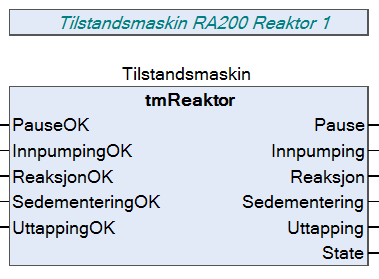
\includegraphics[width=0.4\textwidth]{Bilder/Tilstandsmaskin.png}
    \caption{Tilstandsmaskin implimentert i programmet}\label{fig:reaktorsoner}
\end{figure}


